%
% $RCSfile: pattern_systematics.tex,v $
%
% Copyright (C) 2002-2008. Christian Heller.
%
% Permission is granted to copy, distribute and/or modify this document
% under the terms of the GNU Free Documentation License, Version 1.1 or
% any later version published by the Free Software Foundation; with no
% Invariant Sections, with no Front-Cover Texts and with no Back-Cover
% Texts. A copy of the license is included in the section entitled
% "GNU Free Documentation License".
%
% http://www.cybop.net
% - Cybernetics Oriented Programming -
%
% http://www.resmedicinae.org
% - Information in Medicine -
%
% Version: $Revision: 1.1 $ $Date: 2008-08-19 20:41:08 $ $Author: christian $
% Authors: Christian Heller <christian.heller@tuxtax.de>
%

\subsection{Pattern Systematics}
\label{pattern_systematics_heading}
\index{Pattern Systematics}
\index{Software Pattern}
\index{Object Oriented Programming}
\index{OOP}
\index{Architectural Pattern}
\index{Design Pattern}
\index{Idiomatic Pattern}
\index{Human Thinking}
\index{Discrimination}
\index{Categorisation}
\index{Composition}
\index{Associations within Patterns}
\index{Itemisation Patterns}
\index{1:1 Association Patterns}
\index{1:n Association Patterns}
\index{Recursion Patterns}
\index{Bidirectionalism Patterns}
\index{Polymorphism Patterns}
\index{Grouping Patterns}
\index{Global Access Patterns}

\emph{Software Patterns} (section \ref{pattern_heading}) are a popular
architecture instrument of current systems and languages -- in the first line,
however, of \emph{Object Oriented Programming} (OOP) (section
\ref{object_oriented_programming_heading}). They describe design solutions that
belong to a higher conceptual level, as opposed to the programming paradigms
which are inherent to languages. A common criticism on the existence of
patterns is put into words by the free \emph{Wikipedia} encyclopedia
\cite{wikipedia} which writes:

\begin{quote}
    Some feel that the need for patterns results from using computer languages
    or techniques with insufficient abstraction ability. Under ideal factoring,
    a concept should \emph{not} be \emph{copied}, but merely \emph{referenced}.
    But if something is referenced instead of copied, then there is no pattern
    to label and catalog.
\end{quote}

In other words, patterns would become superfluous, if they could be applied
just \emph{once} to a system, in a manner that allowed any other parts of that
system to reference and reuse-, instead of copy them.

\emph{Cybernetics Oriented Programming} (CYBOP) wants to eliminate the need for
repeated pattern usage, and such enable application programmers, and possibly
even domain experts, to faster create better application systems. On the way to
reaching such sublime aims, a first step is to look at current pattern solutions
and try to identify what their common characteristics are. This was already
done in section \ref{pattern_heading}, which used traditional proposals
\cite{buschmann, gamma1995} to systematise patterns and divided them according
to the first categorisation level shown in figure \ref{pattern_figure}, into
\emph{Architectural-}, \emph{Design-} and \emph{Idiomatic} patterns.

This section proposes a \emph{new} systematics to classify software patterns.
It is based on the idea of classifying them after the principles of
\emph{Human Thinking}, as described in section \ref{human_thinking_heading}
before. These fundamental principles are: \emph{Discrimination},
\emph{Categorisation} and \emph{Composition}. Applied together, they may form
an abstract \emph{Schema} (introduced later, in section \ref{schema_heading}).

The latter two activities of abstraction -- categorisation and composition --
are based on special \emph{Associations} (figure \ref{abstraction_figure}),
between a \emph{Super-} and a \emph{Sub} model and between a \emph{Whole-} and
a \emph{Part} model, respectively. Most patterns heavily rely on associations,
too. This work therefore suggests to \cite{heller2005}: \textit{Take the kind
of association as criterion to sort patterns in a completely new way.}

\begin{table}[ht]
    \begin{center}
        \begin{footnotesize}
        \begin{tabular}{| p{20mm} | p{20mm} | p{50mm} | p{10mm} |}
            \hline
            \textbf{Category} & \textbf{Equivalent} & \textbf{Representative} & \textbf{Advice}\\
            \hline
            Itemisation & Discrimination & Command, Data Transfer Object, State, Memento, Envelope-Letter, Prototype & \vfill 
\includegraphics[scale=0.025,angle=-90]{graphic/happysmiley.pdf}\\
            \hline
            1:1 Association & Composition & Delegator, Object Adapter, Proxy (Surrogat, Client-/ Server Stub), Wrapper, Handle-Body, Bridge & \vfill 
\includegraphics[scale=0.025,angle=-90]{graphic/happysmiley.pdf}\\
            \hline
            1:n Association & Composition & Whole-Part, View Handler, Broker (Mediator), Master-Slave, Command Processor, Counted Pointer, Chain of Responsibility & \vfill 
\includegraphics[scale=0.025,angle=-90]{graphic/happysmiley.pdf}\\
            \hline
            Recursion & Composition & Composite, Interpreter, Decorator, Linked Wrapper & \vfill 
\includegraphics[scale=0.025,angle=-90]{graphic/happysmiley.pdf}\\
            \hline
            Bidirectionalism & -- & Observer (Callback, Publisher-Subscriber), Forwarder-Receiver, Chain of Responsibility, Visitor, Reflection & \vfill 
\includegraphics[scale=0.025,angle=-90]{graphic/sadsmiley.pdf}\\
            \hline
            Polymorphism & Categorisation & Template Method, Builder, Factory Method, Class Adapter, Abstract Factory (Kit), Strategy (Validator, Policy), Iterator (Cursor) & \vfill 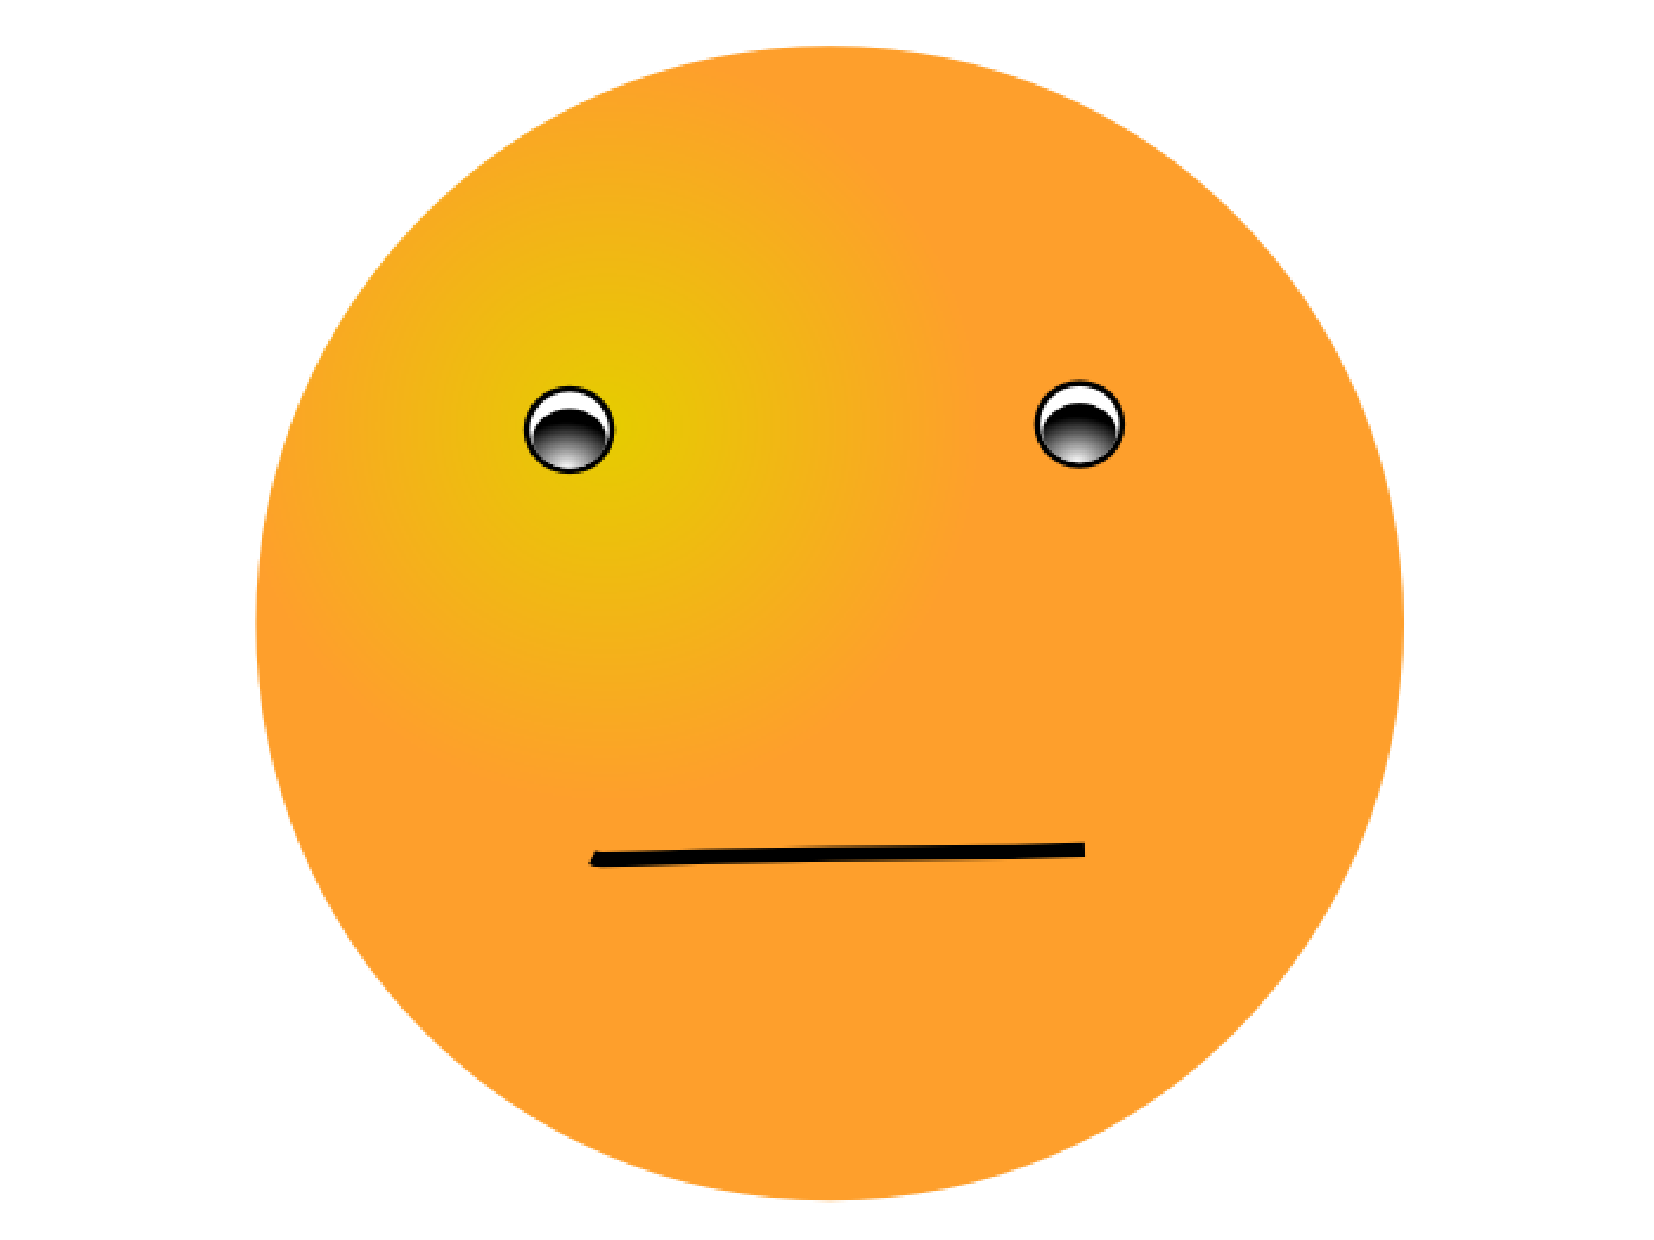
\includegraphics[scale=0.025,angle=-90]{graphic/serioussmiley.pdf}\\
            \hline
            Grouping & Categorisation & Layers, Domain Model, MVC & \vfill 
\includegraphics[scale=0.025,angle=-90]{graphic/happysmiley.pdf}\\
            \hline
            Global Access & -- & Singleton, Flyweight, Registry, Manager & \vfill 
\includegraphics[scale=0.025,angle=-90]{graphic/sadsmiley.pdf}\\
            \hline
        \end{tabular}
        \end{footnotesize}
        \caption{Pattern Systematics}
        \label{pattern_systematics_table}
    \end{center}
\end{table}

Table \ref{pattern_systematics_table} shows a systematics of the new pattern
categories with their equivalents in human thinking, some representative
example patterns and a recommendation for their usage in software engineering.
Patterns matching into more than one category are placed after the priority:
\emph{Recursion} over \emph{Polymorphism}.
